\documentclass{standalone}
 
\usepackage[tikz,math]{forsyde}

\newsavebox{\plots}
\savebox{\plots}{
  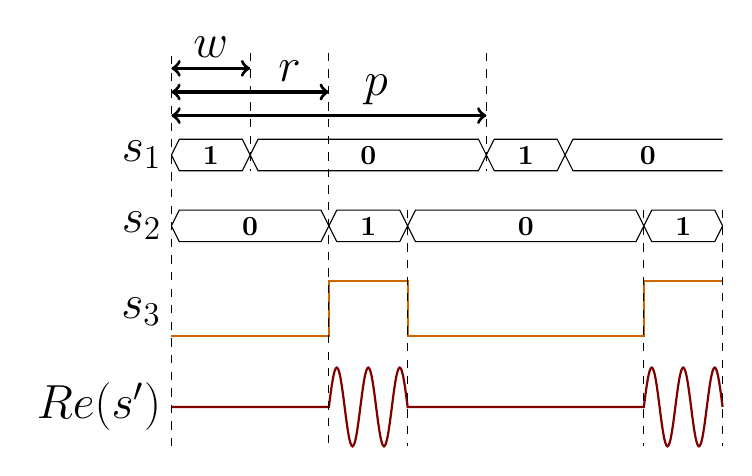
\begin{tikzpicture}[delb/.style={midway,anchor=south,inner sep=2pt}]
    \draw[thick,red!50!black]
    % 2-3,6-7
    (0,0) node[anchor=east,black] (o1) {\LARGE$\operatorname{Re}(s')$}
    (o1.east)--++(2,0)
    sin (2.1,.5) cos (2.2,0) sin (2.3,-.5) cos (2.4,0)
    sin (2.5,.5) cos (2.6,0) sin (2.7,-.5) cos (2.8,0)
    sin (2.9,.5) cos (3,0)
    --++(3,0)
    sin (6.1,.5) cos (6.2,0) sin (6.3,-.5) cos (6.4,0)
    sin (6.5,.5) cos (6.6,0) sin (6.7,-.5) cos (6.8,0)
    sin (6.9,.5) cos (7,0)
    ;
    \draw[thick,orange!80!black]
    % 2-3,6-7
    (0,.9) node[anchor=south east,black] (o1) {\LARGE$s_3$}
    (o1.south east)--++(2,0)--++(0,.7)--++(1,0)--++(0,-.7)
    --++(3,0)--++(0,.7)--++(1,0)
    ;
    \draw
    % 2-3,6-7
    (0,2.3) node[anchor=east] (o1) {\LARGE$s_2$}
    (o1.east)--++(.1,.2)--++(1.8,0)--++(.1,-.2) coordinate (o2)
    (o1.east)--++(.1,-.2)--++(1.8,0) node[delb] {\bf 0} --++(.1,.2)
    (o2)--++(.1,.2)--++(.8,0)--++(.1,-.2) coordinate (o3)
    (o2)--++(.1,-.2)--++(.8,0) node[delb] {\bf 1} --++(.1,.2)
    (o3)--++(.1,.2)--++(2.8,0)--++(.1,-.2) coordinate (o4)
    (o3)--++(.1,-.2)--++(2.8,0) node[delb] {\bf 0} --++(.1,.2)
    (o4)--++(.1,.2)--++(.8,0)--++(.1,-.2)
    (o4)--++(.1,-.2)--++(.8,0) node[delb] {\bf 1} --++(.1,.2)
    ;
    \draw
    % 0-1,4-5,7
    (0,3.2) node[anchor=east] (o1) {\LARGE$s_1$}--++(.1,.2)--++(.8,0)--++(.1,-.2) coordinate (o2)
    (o1.east)--++(.1,-.2)--++(.8,0) node[delb] {\bf 1} --++(.1,.2)
    (o2)--++(.1,.2)--++(2.8,0)--++(.1,-.2) coordinate (o3)
    (o2)--++(.1,-.2)--++(2.8,0) node[delb] {\bf 0} --++(.1,.2)
    (o3)--++(.1,.2)--++(.8,0)--++(.1,-.2) coordinate (o4)
    (o3)--++(.1,-.2)--++(.8,0) node[delb] {\bf 1} --++(.1,.2)
    (o4)--++(.1,.2)--++(1.9,0)%--++(.1,-.2)
    (o4)--++(.1,-.2)--++(1.9,0) node[delb] {\bf 0} %--++(.1,.2)
    ;
    \draw[dashed,thin](0,-.5) to (0,4.5) (1,4.5) -- (1,3) (4,4.5) -- (4,3)
    (2,4.5) -- (2,-.5) (3,2.5) -- (3,-.5) (6,2.5) -- (6,-.5) (7,2.5) -- (7,-.5); 
    \draw[<->,very thick] (0,3.7)--++(4,0) node[midway,anchor=south,xshift=6mm] {\LARGE$p$};
    \draw[<->,very thick] (0,4.0)--++(2,0) node[midway,anchor=south,xshift=5mm] {\LARGE$r$};
    \draw[<->,very thick] (0,4.3)--++(1,0) node[midway,anchor=south] {\LARGE$w$};
  \end{tikzpicture}
}

\begin{document}
\begin{tikzpicture}
  \standard[process,moc=de,f={1;$w$;$p$},type=pwm](pwm)<0,0>{};
  \standard[process,moc=ct,f={$(I+iQ)(t)$},type=infinite,%
    anchor=west,yshift=1.5cm](env)<pwm.west>{};
  \basic[primitive,right of=pwm,xshift=.5cm](refl){$\MocDel$};
  \interface[right of=refl,xshift=.5cm](if){de}{ct};
  \basic[primitive,xshift=2cm,f=$\times$](comb)<$(if)!.5!(env)$>{$\MocCmb$};
  \cluster[farmstyle,type=farm,inner sep=10pt,f=$N_A$](frm)<(env)(pwm)(comb)>{objectReflection};
  
  \gettikzx{(if.east)}{\x};
  \gettikzy{(env)}{\y};
  \path[s=de] (refl) edge[<-] (pwm) edge[->] (if);
  \path[s=ct] (\x,\y) edge[-] (env)
  (comb) edge[<-] (\x,\y) edge[<-] (if.east) edge[trans={s}{frm-east}{v,->}] ++(1.2,0);

  \node[anchor=south west] at (pwm.east) {$s_1$};
  \node[anchor=south west] at (refl.east) {$s_2$};
  \node[anchor=west] at (if.east) {$s_3$};
  \node[anchor=south west,inner xsep=1pt] at (comb.east) {$s'$};

  \node[anchor=west,scale=.56] at (frm.east) {\usebox{\plots}};
\end{tikzpicture}
\end{document}

%%% Local Variables:
%%% TeX-command-default: "Make"
%%% mode: latex
%%% TeX-master: "../journal"
%%% End:
